\chapter{Write Away 8}

\begin{figure}[H]
    \centering
    \includegraphics[width=\textwidth/2]{./Games/WriteAway/Images/WriteAway8CD.png}
    \caption{Write Away 8 CD}
\end{figure}

The eigth of the ten Write Away games published and released by The Lightspan Partnership for the PlayStation 1.

Write Away 8 features nine video programs, including an introduction video, seven story videos, and a conclusion video:

\begin{itemize}
    \item Write Away Episode Eight Introduction
    \item Tracks in the Snow by Marci Rivera
    \item The Magic Ring by Aimee Lewis \& Nichole Potts
    \item A Young Woman Named Harris by Ashlee Dugger
    \item My Funny Friend \& My Special Cousin by Jeremy Begay \& Julius Martinez
    \item The Castle by Matt Manning
    \item Our School Community by Sarah Tavarez
    \item Best Friends by Madiata Messo
    \item Write Away Conclusion
\end{itemize}

\clearpage
\newpage

\section{Transcriptions}

\subsection{Tracks in the Snow by Marci Rivera}

JENNIFER:
Welcome back to Write Away, a show written by students just like yourselves from all over the country.
With tools as simple as a pencil, or as fancy as a computer, you can let your imaginations flow onto the paper to create funny, sad, exciting, or even scary stories.
You can paint pictures with your words so that people will be able to visualize just what you're imagining.
A good example of this is our first story today.
She's a student at Conti School in New Jersey, and her story is called 'Tracks in the Snow'.
After it snows, it's fun to walk through the woods and guess who or what made all those tracks.
Come on, let's take a look.

JENNIFER (VOICE OVER):
This was a mouse who played by himself, dancing left and right under the winter moon.
And over here, look at this track!
And this track must have been a pheasant walking to meet a friend.

Look, this one's easy.
This is a rabbit running very fast, the way all rabbits do.
And I definitely know what this track is: a squirrel who was happy finding a nut.
And this uncommon track is probably me.
Tracks in the Snow.
The end.

\subsection{The Magic Ring by Aimee Lewis \& Nichole Potts}

PAUL:
Get out of my way, you crocodiles!
I'm coming through.
    [Get out] -
Oh, hello!
I was just imagining I was going down the Amazon in a canoe.
I love adventure stories.
What's great about writing adventure stories is you can stay in the safety of your own room by experiencing all the thrills and dangers that come pouring out of your pencil.
Our next authors share their exciting exploits with us as their main character goes through some unusual adventures for the surprise ending.
Our authors come from Apalachee School in Tallahassee, Florida.
Come with me as we see what Aimee Lewis and Nichole Potts have dreamed up for us in 'The Magic Ring'.

NARRATOR:
Once there was a girl named Marie who wanted to be an explorer.

MARIE:
Hey, you guys, I just saw a shooting star!

GIRL 1, GIRL 2, BOY 1:
Wow!

MARIE:
Yeah, someday, when I grow up, I'll be an explorer, and I'm gonna visit all those countries, like the ones on those maps.

BOY 1:
Girls can't be explorers.

MARIE:
Yes, they can!

GIRL 1:
Oh yes, they can!

GIRL 2:
Can.

MARIE:
You'll see.

GIRL 1:
Yeah, you'll see.

GIRL 2:
See.

NARRATOR
One day, Marie went into the forest pretending to be an explorer.

MARIE:
Follow me, men and women, as we go on our journey, climbing over the mountains, through the river.
Watch out!
There's a crocodile.
Stand back, I'll get it.
Come here you.
Boop!
You had enough?
Get out of here!
And now, to find the Lost Treasure of Atlantis!
Hey!
What's that?

NARRATOR:
Suddenly, Marie saw something shiny on the ground.
It was a beautiful ring.

MARIE:
Ooh, I did find a treasure!
This ring is beautiful.
I'm sure no one would mind if I just tried it on.

NARRATOR:
Marie slipped the ring on her finger.
It was a perfect fit.
But suddenly, Marie began to feel strange.

MARIE:
Ooh!
What's happening?
I feel odd!

NARRATOR:
Marie suddenly turned into a bunny.
And then an alligator
And then a ferocious dog

MARIE:
Ruff, ruff, ruff!

NARRATOR:
And finally, a monkey.

MARIE:
*monkey noises*
Oh no, the ring!
It blew off!
It's lost!
I guess I'll have to stay this way forever!
*monkey noises*

BOY:
Here's another banana, Marie.

MARIE:
*monkey noises*

BOY:
Don't worry.
You\dots look good that way.

GIRL 1:
Yeah, real good.

GIRL 2:
Good.

MARIE:
Thanks you guys, I\dots
I'm not gonna let this little setback get me down.
You know, someday, I am going to be an explorer, because I want to know what's out there.

NARRATOR:
And so, Marie, who wanted to be an explorer, got the adventure of her life.
The End.

\subsection{A Young Woman Named Harris by Ashlee Dugger}

SCOUT:
June, moon, spoon tune.
I like to rhyme, so of course I like poetry.
And one kind of poetry that I really like is called a limerick.
A limerick is a very specific type of poem that's named after the Irish County of Limerick in Ireland.
In a limerick, there are only five lines, and it's usually very funny.
Ashlee Duggar, a student at Martin Luther King School in San Diego, California, brings to us a wonderful limerick that she's entitled 'A Young Lady Named Harris'.

JENNIFER (VOICE OVER):
There was a young lady named Harris, who, nothing could ever embarrass.

BOY:
You know, I just hate blind dates, don't you, haha!
Okay, let's dig in!
[I love it].
*food in his mouth* This tastes very good.
I love it.
*inaudible sounds from food in his mouth*
Goo- goo-  goodnight.
That's good, I love it.

GIRL:
Goodnight\dots
I need a nice hot bath after a date like that.

JENNIFER (VOICE OVER):
Till that one fateful day, the bath salts she mislaid.
And now she's in plaster of Paris.

GIRL:
Help!

\subsection{My Funny Friend \& My Special Cousin by Jeremy Begay \& Julius Martinez}

SABRINA:
Here's some good advice for you authors who might be having a hard time getting your story started.
Why not try what two of our authors have done?
They each started with someone they already knew really well, and through their writing helped share their special relationship.
Their names are Jeremy Begaye and Julius Martinez.
They both attend Ojo Amarillo School in Fruitland, New Mexico.
Jeremy shares with us 'My Funny Friend Xavier', and Julius tells us about 'My Special Cousin'.

JENNIFER:
And so, that's how you build a grandfather clock.

TEACHER:
Oh, thank you, Jennifer.
Yes, very good.
Now for our next assignment, I want you to get out your pencils and your papers, and we're going to write about someone or something that's very special to us.
For example, my little parakeet Sweetie Pie is very special to me.
All right, everybody, begin.

GIRL (VOICE OVER):
I'll write about my mother.

JENNIFER (VOICE OVER):
I'll write about my dog.

BOY 1 (VOICE OVER):
I wonder what's for lunch.

TEACHER:
I think I'll go bungee jumping this weekend.

BOY 2:
I know, I'll write about my favorite cousin.

BOY 2 (VOICE OVER):
When I was three, I met him at the fair.
I heard his happy laugh.
Then I saw him at the mall, and I felt as happy as a cat.
Then we went swimming.
And then we had a party.

BOY 2:
My special cousin.
The end.

GIRL 1 (VOICE OVER):
I'm almost done.

JENNIFER (VOICE OVER):
When's lunch?

TEACHER (VOICE OVER):
I think I'll learn to surf.

BOY 1:
I know, I'll write about my funny friend Xavier.

BOY 1 (VOICE OVER):
When I was four, I met Xavier at school.
I liked his laugh.
We went to the mall, and I felt as happy as a cat.
And then we went to the movies.

BOY 1:
I really like my funny friend Xavier.
The end.

TEACHER:
All right, everybody, time's up.
Turn in your papers and have fun and go to lunch!
Yes, here we go, very good.
Ooh, oh my.
Let's see, what did they have here?
Yes, oh, 'My Special Cousin.'
Oh, that sounds good, and, 'My Funny Friend Xavier.'
Ho, they sound wonderful!
Oh, I just can't wait to read them.

\subsection{The Castle by Matt Manning}

JOE:
One thing that I like about writing is that I am totally in charge.
I could write about any character and put them in any situation.
I could even give my main character something he thought was really great, but turned out to be a nightmare.
Our next author uses this concept to create a unique tale.
Matt's story is called 'The Castle'.

MAN:
One day I was just reading when the mail came, as usual.

MAILMAN:
Mail!

MAN:
Thanks.
Junk mail, junk mail, junk mail...
Woah.
But that's when I saw it.
Some crazy bank gave me a credit card!
Duh!
I think I'll go shop till I drop.
Ah ha ha!

MAN (VOICE OVER):
But then I got the bill.

MAILMAN:
Mail.

MAN (VOICE OVER):
And I fainted.

MAN:
Oh\dots
What is this?
Where am I?
Stone walls, a drawbridge\dots
This must be a castle.
What does that sign say?
'Castle of War'.
Oh no!
I must have traveled back in time, and now I'm at a medieval castle!
I'm gonna walk around and check things out.
I've gotta find a way back home.
Woah, that guard keeps staring at me.
Oh no!

GUARD:
Intruder!
Intruder!
Capture the intruder!

MAN:
No time to think, got to run!
Excuse me.
Where am I?

GUARD:
Yo, in the kitchen of the Castle of War.
I'm the cook who cooks in the kitchen of the Castle of War.
*spit*

MAN:
Eugh.
What do you cook?

COOK:
Well, here in the kitchen of the Castle of War, we cook cabbage, meat, vegetables, potatoes, and intruders.

MAN:
Oh, you mean like me?

COOK:
Intruder!

MAN:
Augh, thanks a lot.
Woah, I'll be safe in here.
Oh, it's a dungeon.
No time to panic, no time to panic.
Panic!
Panic!

GUARD 2:
Quiet, intruder!
Eat this cabbage from the cook of the kitchen of the Castle of War, for tomorrow will be your last.
Hahaha!

PRISONER:
Psst.
Whatever you do, don't eat the cabbage from the cook of the kitchen of the Castle of War.

MAN:
Why not dude?

PRISONER:
You'll find out.

MAN:
Eugh, bony.
Well who are you?

PRISONER:
I'm the cousin of the cook of the kitchen of the Castle of War.

MAN:
Cousin Cook Castle War, whatever, dude.
I'm hungry.

MAN (VOICE OVER):
So, I began to eat my food in a panicked manner.
*begins to choke*
I'm choking, I'm choking!

GUARD 1:
He's choking!

COOK:
He's choking!

GUARD 2:
He's choking!

GUARD 1, GUARD 2, COOK:
He's choking!

MAN:
Help!
Help!
Woah!
I'm back home.
And I'm not choking.
Woah, what a terrible dream.
I've learned my lesson well.
I will never use a credit card again if I don't have the money to pay for it.
Haha.
Never give kids credit cards.

MAILMAN:
Mail.

MAN:
Thanks.
Junk mail, junk mail, credit c- credit card!

\subsection{Our School Community by Sarah Tavarez}

JENNIFER:
One form of writing is a Chronicle, which is a record of events.
This helps the reader to see how something was accomplished.
Our next writer utilizes this form of writing to show how teamwork can achieve anything.
Sarah Tavarez attends Helen Ball School in El Paso, Texas.
She shares with us a picture of what it's like at her school, where they all work together in 'Our School Community'.

GIRL 1 (TO VIEWER):
Our school community works as a team.

EVERYONE:
Yeah!

GIRL 1 (TO VIEWER):
Every day we do reading and spelling, with students leading students.

GIRL 2:
And then the ball went -

BOY 1:
- into the hole.

GIRL 2:
Very good!

GIRL 1 (TO VIEWER):
Our students get along with each other and encourage each other to do their best!

BOY 1:
Come on, you can do it!
You can do it!
All right!

GIRL 1:
Thanks, I did it!

GIRL 1 (TO VIEWER):
We clean up our classroom and share school supplies.
The teachers in our school work as a team too.
They plan, support, and give each other ideas.

TEACHER 1:
You know what?
I'm gonna take my kids to the zoo.

TEACHER 2:
Ah, I think I'll take my class with yours, and I'll drive the bus, and I'll make all the lunches!

TEACHER 1:
And I'll make the name tags.
Oh, let me grade those papers for you.

TEACHER 2:
Let's grade them together!

GIRL 1 (TO VIEWER):
So now you see how everyone at school should work as a team, and that's our school community at Helen Ball Elementary.

EVERYONE:
Bye!

\subsection{Best Friends by Madiata Messo}

PAUL:
Oh hi!
I was just reading some Aesop fables.
I love stories that have morals in them because they teach you lessons that you can use for your life.
Now it's not easy to write a story that is both entertaining and inspiring, but Madiata Messo has managed to do just that.
Madiata goes to Mohawk Elementary School in Texas, and she has written an amusing story that has an important message for us.
It is called 'Best Friends'.

NARRATOR:
Once upon a time, there were two boys, Ben and Johnny, who loved music and loved to sing.

BEN:
Hey, hey Johnny.

JOHNNY:
Yeah?

BEN:
Listen to the song I wrote for the big new singing competition.

JOHNNY:
Okay.

BEN:
*singing*
My heart is broken now you're gone.
How can I go on?
Thump, thump, thump, oooooooh!

JOHNNY:
Hehehe!
Manly, yes, but I liked it too!

BEN:
Yeah!

JOHNNY:
Hey, listen to mine.

*singing*
There's a toad in the road, carrying a heavy load.
Don't worry, little toad, watch out for that truck.
Whoa, too bad, little toad!

BEN:
Woah, awesome!

JOHNNY:
Yeah!

BEN:
Hey, but I think we should write an upbeat song for the competition.

JOHNNY:
Yeah, you're right.
Let's begin.

NARRATOR:
Now, the one problem the two boys had was Rob the Bully.
He was jealous of Johnny and Ben.

ROB:
Listen to those two.
They think they're so good just because they can sing.
Well, they can't sing.
They didn't ask me to sing with them, and I'm gonna tell them.
Hey, you guys can't sing because you stink!

JOHNNY:
No, we don't!
Do we?

BEN:
No.

JOHNNY:
No, we don't!
Hey, and don't bother us, man, we're working on the big singing competition.
First prize is a record contract.

BEN:
Yeah, that's right!
You're just jealous you can't sing.
Go away, we need to practice.

JOHNNY:
Yeah, you are disturbing our creative flow.

ROB:
Fine, I'll go.
So-rry.

*to viewer*
I'm gonna ruin their chances of winning, just you wait.

NARRATOR:
Rob the bully put his plan into action.
First, he threw water at them.

BEN:
Hey, is it starting to rain?

JOHNNY:
I don't know.
You better go inside.
We don't want to catch a cold.

BEN:
Yeah.

JOHNNY:
Yeah.

ROB:
I must succeed.
I've got it!
Haha.

NARRATOR:
Rob rubbed soap on the floor to make it slippery.

ROB:
*to viewer* They'll walk on this floor, slip, and be out of the contest!
Mwhahaha.

ROB:
*falls to the floor*
Eugh, my arm!
My back!

*to viewer*
I got it!
Mwhahaha!

NARRATOR:
Rob snuck into the house and took Ben and Johnny's guitars.

ROB:
*to viewer*
Without their instruments, they won't be able to play, and they'll have to forfeit the contest.
Mwhahaha!

JOHNNY:
Oh, bad dream.

BEN:
Ah, woah, who stole my guitar?

JOHNNY:
Ah, and mine!

BEN, JOHNNY:
Rob!

NARRATOR:
Finally, the big day had come.
The contest was in progress.

SINGER 1:
I'm flying high in the sky, and so goodbye!
Thank you, thank you, thank you.

JUDGE:
Thank you.
Thank you, that was great.
And for our last contestants, we have the singing team of Ben and Johnny!

ROB:
You guys will never win.
You don't have any instruments!
Mwhahaha!

JOHNNY:
We don't need instruments because we have the music in our minds.

BEN:
Yeah.

JOHNNY:
A one, a two, a one, two, three, four!

BEN, JOHNNY:
*singing*
We hear the music in our ears, we hear the music through our tears, we hear the music in our toes, but where it comes from, no one knows.
We hear the music in our ears, we hear the music through our tears, we hear the music in our toes, but where it comes from, no one knows.

JUDGE:
That was amazing!
Oh\dots
And the winners are\dots
Ben and Johnny!

BEN, JOHNNY:
Yeah!

JUDGE:
Congratulations!

BEN, JOHNNY:
Thanks.

ROB:
Congratulations, you guys were awesome.
I guess I did all that stuff to you because I was jealous.
Sorry for what I did.

JOHNNY:
It's okay.
Hey, you want to be our road manager?

ROB:
Sure.

BEN:
Yeah, yeah, and you can be a backup singer, and you too, judge lady person.

BEN, JOHNNY:
*singing*
We hear the music in our ears, we hear the music through our tears\dots

NARRATOR:
And so, Ben and Johnny became famous singers and had fun singing all over America.
The end.

BEN, JOHNNY:
*singing*
You're the music in our ears, we hear the music in our tears, we hear the music in our toes, but where it comes from, no one knows.
We hear the music in our ears, we hear the music through our tears, we hear the music in our toes, but where it comes from, no one knows.
Yeah, yeah!

\subsection{Write Away Conclusion}

JENNIFER:
We hope you've enjoyed our show today.
Your stories are finished and all put away.

JOE:
But we'll come again another day.

SCOUT:
The stories you've seen through music and [mime].

SABRINA:
Can be written by you if you just take the time.

PAUL:
So pick up a pencil and paper, you'll see,

EVERYONE:
The adventures and magic that writing sets free.
So, write away!

\section{Credits}

Executive Producers: Gregg Baker, Deborah Brucher Wren, Michael Wren;
Directors: Gregg Baker, Robin LeValley;
Technical Director: Joseph S. Abreu;
Cast: Paul David, Scout Jackson, Joe Lopez, Jr., Sabrina Lu, Jennifer Shelton;
Writers: Deborah Brucher Wren, Robin LeValley;
Music: Rick Illes, Michael Wren;
Lighting Director: Steve Raines;
Cameras: Steve Raines, Andy Hall, Richard Crow;
Audio: Rad Corn;
Childrens Art: Blythe Baker;
Special Costume Design: Dianne Brucher;
Editor: Joseph S. Abreu;
Engineer: Michael Curran;
Production Coordinator: Judy Block;
Graphic Artist: Alan Scott;
Theme Song: Michael Wren;

\clearpage
\newpage

\section{Screenshots}

\begin{figure}[H]
    \centering
    \begin{subfigure}{0.45\textwidth}
        \centering
        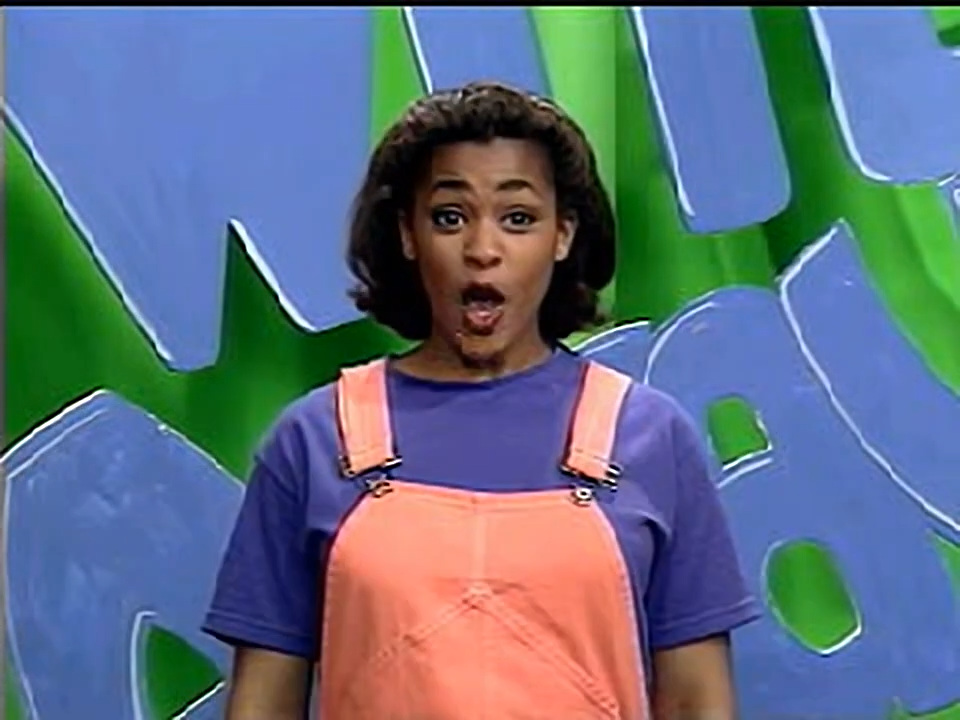
\includegraphics[width=\linewidth]{Games/WriteAway/Images/WriteAway8Screenshot1.png}
        \caption{Write Away 8 - Screenshot 1}
    \end{subfigure}
    \begin{subfigure}{0.45\textwidth}
        \centering
        
\includegraphics[width=\linewidth]{Games/WriteAway/Images/WriteAway8Screenshot2.png}
        \caption{Write Away 8 - Screenshot 2}
    \end{subfigure}

    \begin{subfigure}{0.45\textwidth}
        \centering
        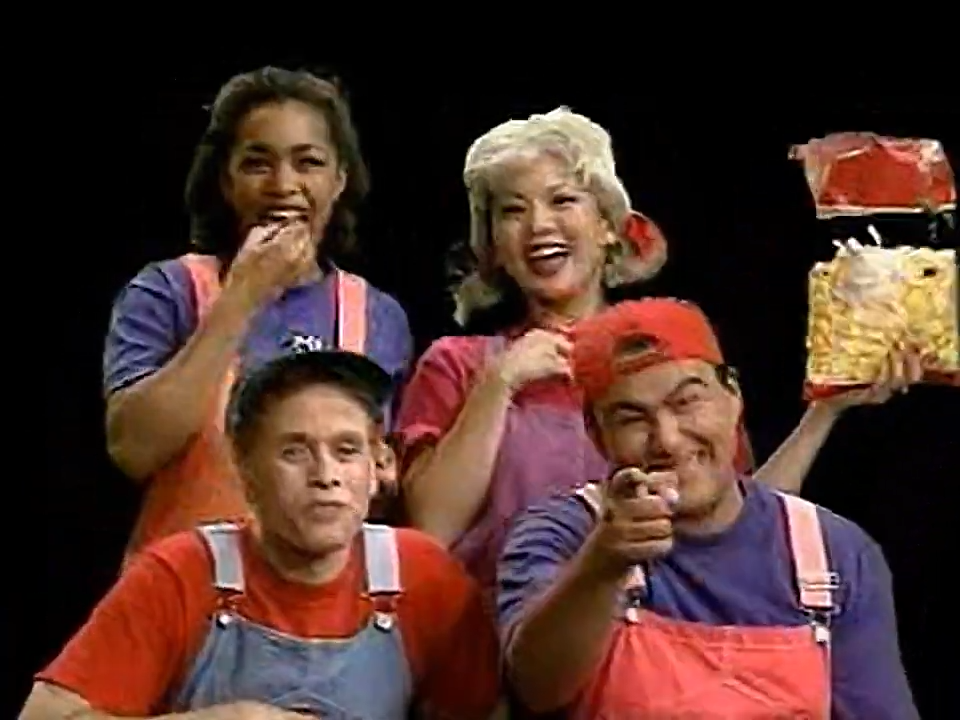
\includegraphics[width=\linewidth]{Games/WriteAway/Images/WriteAway8Screenshot3.png}
        \caption{Write Away 8 - Screenshot 3}
    \end{subfigure}
    \begin{subfigure}{0.45\textwidth}
        \centering
        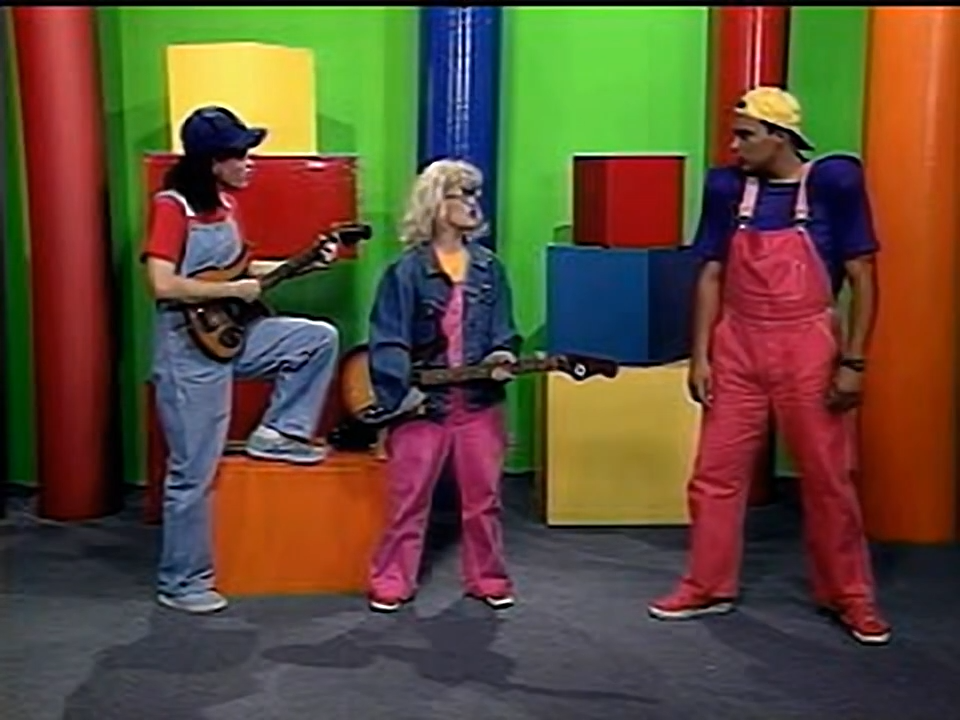
\includegraphics[width=\linewidth]{Games/WriteAway/Images/WriteAway8Screenshot4.png}
        \caption{Write Away 8 - Screenshot 4}
    \end{subfigure}
    \caption{Screenshots from Write Away 8}
\end{figure}
